\documentclass{article}
\usepackage{amsmath,amsfonts,times}
\usepackage{tikz, color, graphicx}
\usepackage[paperwidth=12.0cm,paperheight=6.50cm,lmargin=0in,rmargin=0pt,tmargin=4pt,bmargin=0.in]{geometry}
\usetikzlibrary{arrows,shadings,shapes.arrows,decorations.pathreplacing,calc, positioning}


\begin{document}

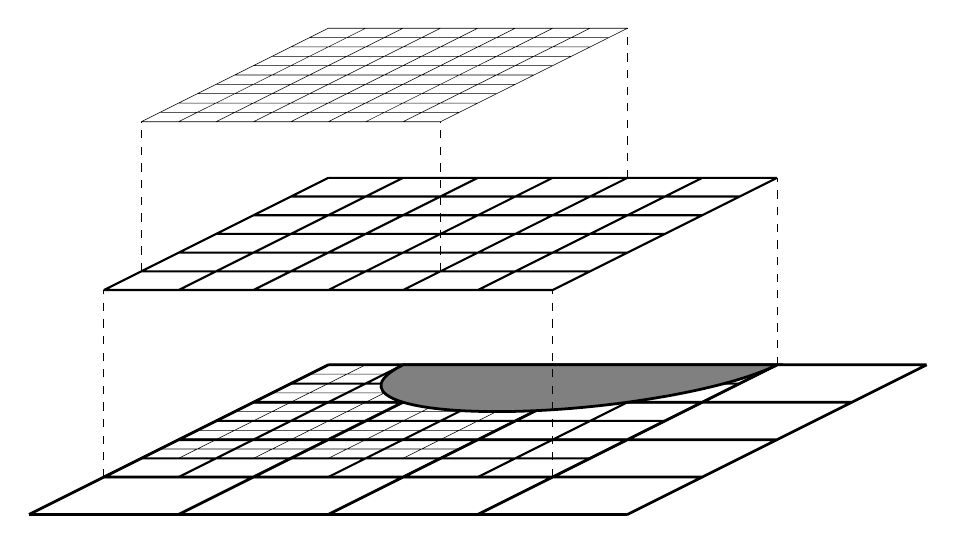
\begin{tikzpicture}[scale = 0.95]
  \draw[yshift=0.0cm, xslant=2., yscale=0.25, line width = 1.00pt, scale = 1, draw=black] (0,0.000) grid[step=2.0] (8,8); % Bottom grid coarse grid
  \draw[yshift=0.0cm, xslant=2., yscale=0.25, line width = 0.75pt, scale = 1, draw=black] (0,2.000) grid[step=1.0] (6,8); % Bottom refined grid 1
  \draw[yshift=0.0cm, xslant=2., yscale=0.25, line width = 0.20pt, scale = 1, draw=black] (0,2.999) grid[step=0.5] (4,8); % Bottom refined grid 2
  
  \draw[yshift=2.5cm, xslant=2., yscale=0.25, line width = 0.75pt, scale = 1] (0,2.000) grid[step=1.0] (6,8); % Middle grid
  \draw[yshift=4.5cm, xslant=2., yscale=0.25, line width = 0.20pt, scale = 1] (0,2.999) grid[step=0.5] (4,8); % Top grid

  \draw[xslant = 2, yscale = 0.25,fill=black!50!white, draw=black, line width = 1pt] (4,8) -- (6,8) arc(0:-180:2.5) --cycle; % EB

  % Lines middle to bottom
  \draw[dashed] (1,0.5) -- (1,3);
  \draw[dashed] (7,0.5) -- (7,3);
  \draw[dashed] (10,2) -- (10,4.5);

  % Lines top to middle
  \draw[dashed] (1.5,3.25) -- (1.5,5.25);
  \draw[dashed] (5.5,3.25) -- (5.5,5.25);
  \draw[dashed] (8.0,4.5) -- (8.0,6.5);

\end{tikzpicture}
\end{document}


